%-----------------------------------------------------------------------------
% CONFIGURE DOCUMENT
%-----------------------------------------------------------------------------

%\documentclass[letterpaper, 10 pt, conference]{ieeeconf}  % Comment this line out
                                                           % if you need a4paper
\documentclass[letterpaper, 10pt, conference]{ieeeconf}    % Use this line for a4
                                                           % paper

\IEEEoverridecommandlockouts                              % This command is only
                                                          % needed if you want to
                                                          % use the \thanks command
\overrideIEEEmargins
% See the \addtolength command later in the file to balance the column lengths
% on the last page of the document
% The following packages can be found on http:\\www.ctan.org
\usepackage{graphics} % for pdf, bitmapped graphics files
%\usepackage{epsfig} % for postscript graphics files
%\usepackage{mathptmx} % assumes new font selection scheme installed
%\usepackage{times} % assumes new font selection scheme installed
\usepackage{amsmath} % assumes amsmath package installed
\usepackage{amssymb}  % assumes amsmath package installed
\usepackage{url}
\usepackage{graphicx}
\usepackage{listings}
\usepackage{color}

\usepackage{listings}
  \usepackage{courier}
 \lstset{
         %basicstyle=\footnotesize\ttfamily, % Standardschrift
         basicstyle=\scriptsize\ttfamily, % Standardschrift
         %numbers=left,               % Ort der Zeilennummern
         numberstyle=\tiny,          % Stil der Zeilennummern
         %stepnumber=2,               % Abstand zwischen den Zeilennummern
         numbersep=5pt,              % Abstand der Nummern zum Text
         tabsize=1,                  % Groesse von Tabs
         extendedchars=true,         %
         breaklines=true,            % Zeilen werden Umgebrochen
         keywordstyle=\color{red},
            frame=b,
 %        keywordstyle=[1]\textbf,    % Stil der Keywords
 %        keywordstyle=[2]\textbf,    %
 %        keywordstyle=[3]\textbf,    %
 %        keywordstyle=[4]\textbf,   \sqrt{\sqrt{}} %
         stringstyle=\color{white}\ttfamily, % Farbe der String
         showspaces=false,           % Leerzeichen anzeigen ?
         showtabs=false,             % Tabs anzeigen ?
         xleftmargin=17pt,
         framexleftmargin=17pt,
         framexrightmargin=5pt,
         framexbottommargin=4pt,
         %backgroundcolor=\color{lightgray},
         showstringspaces=false      % Leerzeichen in Strings anzeigen ?
 }
 \lstloadlanguages{% Check Dokumentation for further languages ...
         %[Visual]Basic
         %Pascal
         %C
         %C++
         XML
         %HTML
         %Java
 }
    %\DeclareCaptionFont{blue}{\color{blue}}

  %\captionsetup[lstlisting]{singlelinecheck=false, labelfont={blue}, textfont={blue}}
  \usepackage{caption}
    %\DeclareCaptionFont{white}{\color{white}}
    %\DeclareCaptionFormat{listing}{\colorbox[cmyk]{0.43, 0.35,0.35,0.01}{\parbox{\textwidth}{\hspace{15pt}#1#2#3}}}
    \DeclareCaptionFormat{listing}{\colorbox[cmyk]{0.43, 0.35,0.35,0.01}{\parbox{\columnwidth}{\hspace{15pt}#1#2#3}}}
    %\captionsetup[lstlisting]{format=listing,labelfont=white,textfont=white,singlelinecheck=false, margin=0pt, font={bf,footnotesize}}
    \captionsetup[lstlisting]{format=listing,singlelinecheck=false, margin=0pt}

\graphicspath{{./}{./figures/}}

%-----------------------------------------------------------------------------
% TITLE
%-----------------------------------------------------------------------------

\title{\LARGE \bf Architecture and Tools for the Generation of Flight Intent from Mission Intent for a Fleet of Unmanned Aerial Systems}

% \author{ \parbox{3 in}{\centering Huibert Kwakernaak*
%         \thanks{*Use the $\backslash$thanks command to put information here}\\
%         Faculty of Electrical Engineering, Mathematics and Computer Science\\
%         University of Twente\\
%         7500 AE Enschede, The Netherlands\\
%         {\tt\small h.kwakernaak@autsubmit.com}}
%         \hspace*{ 0.5 in}
%         \parbox{3 in}{ \centering Pradeep Misra**
%         \thanks{**The footnote marks may be inserted manually}\\
%        Department of Electrical Engineering \\
%         Wright State University\\
%         Dayton, OH 45435, USA\\
%         {\tt\small pmisra@cs.wright.edu}}
% }

%-----------------------------------------------------------------------------
% AUTHORS and CONTACTS
%-----------------------------------------------------------------------------

\author{Ivan Maza, Jorge Mu\~{n}oz-Morera, Fernando Caballero, Enrique Casado, Victor Perez-Villar and Anibal Ollero   % $<$-this % stops a space
\thanks{This work is partially supported by the ADAM Project funded by the spanish Centre for the Development of Industrial Technology (CDTI), the
ARCAS Project (FP7-ICT-287617) funded by the EU FP7 and the RANCOM Project (P11-TIC-7066).} % $<$-this % stops a space
\thanks{Ivan Maza, Jorge Mu\~{n}oz-Morera, Fernando Caballero and Anibal Ollero
are with the Robotics, Vision and Control Group, University of Seville, Avd. de los Descubrimientos s/n, 41092, Sevilla, Spain. Email:
{\tt\small imaza@us.es, jorgemunoz@us.es, fcaballero@us.es, aollero@us.es}}
\thanks{Enrique Casado and Victor Perez-Villar are with Boeing Research \& Technology Europe, Avenida Sur del Aeropuerto de Barajas 38,
Bldg 4, 28042 Madrid, Spain. Email: {\tt\small Enrique.Casado@boeing.com, victor.perezvillar@boeing.com}}%
%\thanks{A. Ollero is also with the Center for Advanced Aerospace Technology (CATEC), Seville, Spain. Email: {\tt\small aollero@catec.aero}}
}

%-----------------------------------------------------------------------------
% DOCUMENT
%-----------------------------------------------------------------------------
\begin{document}

\maketitle

\thispagestyle{empty}

\pagestyle{empty}

%-----------------------------------------------------------------------------
% ABSTRACT
%-----------------------------------------------------------------------------
\begin{abstract}
Flight intent refers to the information which describes the trajectory to be flown by an aircraft considering the operational context in
which the flight take place and the user preferences to be fulfilled along the whole trajectory. In previous work, the set of rules which
ensures the generation of valid instances of flight intent was structured as a formal language, the Flight Intent Description Language
(FIDL). This paper extends these concepts to a higher level of abstraction, the mission level, and presents the architecture and tools used
to generate flight intent from the mission intent expressed in a formal language. The core component of this architecture is a planner that
takes the mission intent sentences as inputs and computes a high-level plan in a multi-vehicle context to achieve the goals commanded. The
architecture and resulting workflow are illustrated with a surveillance mission to be executed by a fleet of UAS equipped with different
payloads.
\end{abstract}

%-----------------------------------------------------------------------------
% KEYWORDS
%-----------------------------------------------------------------------------

\begin{keywords}
Command and Control; Flight Intent; Multiple UAS; Mission Intent; Autonomy; Interoperability
\end{keywords}

\section{Introduction and Related Work}
\label{sec:intro}

The development of new unmanned platforms capable of performing autonomous operations are nowadays becoming a major research area, especially
those elements related to interoperability among heterogeneous platforms and to autonomous, collaborative and coordinated mission execution.

Regardless the type of vehicle and payload on-board, a clear need for reaching the expected performances is to have a common framework for
design and develop missions which can be also used for control and monitoring purposes. However, currently this basic requirement is solved
individually by each system, defining its own formal structure that is used for generating the mission goals and objectives based on the user
requirements. The common approach is to describe such information in the way that can be communicated to the systems in each native format.
This approach eludes the possibility of sharing information among other systems not compatible with the used framework.

Although Unmanned Aerial Systems (UAS) have been designed and developed for performing military missions, currently the trend is to extend
their applicability to civil mission, such as, firefighting~\cite{merino_jint12}, critical infrastructure protection or remote
surveillance~\cite{acevedo_jint13} among many others. The multiple variety of platform, control system and ground-based equipments, and the
heterogeneity of the communication devices have made difficult the interoperability among the different systems. Each manufacturer has
produced its own infrastructure which manage the information of the mission in a native format. This drawback implies that complex missions
with a broad range of autonomous vehicles are highly complicated for planning, execution and monitoring. This situation provokes that the end
users prefer to have individual systems for each specific mission instead of homogenizing all of them into a common framework. But the
benefits of this common framework are clear: enhanced capabilities because the global system would become more flexible and any new system
could be added without any special complication.

Different related work and initiatives can be found in the last years. Worried about interoperability problems between simulation systems, some
international organizations such as the Simulation Interoperability Standards Organization (SISO) have developed or improved simulation-to-simulation
standards such as Distributed Interactive Simulation (DIS) and High Level Architecture (HLA). In parallel and motivated by the same reasons as the
SISO, the Multilateral Interoperability Programme (MIP) developed the Joint Consultation Command and Control Information Exchange Data Model (JC3IEDM)
as a data model which specifies the minimal data set needed to exchange military information between Command and Control (C2) systems. These works
represent a base solution to achieve interoperability between simulation and C2 systems, but still many systems have a unique interface.

One way to increase the interoperability between C2 system is the use of a Battle Management Language (BML). A BML is an unambiguous language
used in the military field to command and control forces using different types of constructions that lets create orders, reports, request and
other types of necessary information in a way close to the human language. Over the last decades different Battle Management Languages have
been used, allowing to acquire certain degree of technical and operational coherence. Technical coherence refers to the ability of systems to
interconnect and send information that may be parsed and processed between them while operational coherence refers to the ability to share
different conceptual and semantic models of the mission space between systems as a base for an unambiguous communication and control
\cite{SISO-DRAFT}. Different systems that implements or use the same BML could communicate between them. Due to the number of different BML
developed in earlier works and as a way of unification, the SISO proposed the Coalition-Battle Management Language (C-BML) as a standard.

The Coalition-Battle Management Language is based on the JC3IEDM and represent an standard abstraction of the orders that a commander
may make to command real troops, simulated systems or robotics systems. Such orders represent the commander's intent: a clear, concise statement
of what the force must do and the conditions the force must meet to succeed with respect to the enemy, terrain and the desired state, or
by extension, a clear, concise statement of what an organization must do and the conditions it must meet in order to succeed at a task \cite{SISO-DRAFT}.
Although originally intended to military missions, the reference data model is rich enough to additionally use it in civilian missions. Furthermore,
the language is still under development: the first phase � out of three � of the specification was published on April 2012, so the emerging needs during the
development process will be taken into account for the next phases. The language specification is composed by three elements: the Data Model Specification,
the Information Exchange Structure and Content Specification and the Information Exchange Mechanism. The Data Model specification refers to the base
data model and as stated above it's the JC3IEDM. The Information Exchange Structure and Content Specification is composed of two models: the
conceptual model of the language and the structural model of the language. The conceptual model is based on the widely known 5Ws (Who, What,
When, Where and Why) and present the principal information components that compose the different orders, requests and reports that we may make.
The structural model describes the content and structure of the C-BML expression and uses the XML Schema language, so all the expressions are
defined into XML documents that are passed between the different systems. Finally the Information Exchange Mechanism Specification describes how
the information (C-BML expressions) is transferred between systems, and although the formal mechanism will be specified in future phases it seems that
Web Services will be the base for the communication.

In addition to the C-BML development the SISO created the Military Scenario Definition Language (MSDL). The MSDL is an XML language developed with the
purpose of verifying and loading military scenarios in simulation systems, making it possible to reuse and share them between different systems or platforms,
thus reducing the development time and cost. It describes the physical location and configuration of the mission space, including the terrain, weather,
present forces, etc. The language uses some parts of the JC3IEDM related to meteorological and battlespace domains, so it's closely related with C-BML.
In fact both standardization groups are mutually dependent, having each one some members working on the other to improve the development effort. This is
due to the overlapping areas that both languages seem to have: the forces and settings defined in a scenario are used in C-BML expressions and the orders
given in C-BML expressions (such any that implies some kind of troop movements for example) are needed in MSDL for the scenario initialization. That makes
MSDL and C-BML go by the hand.

The Joint Battle Management Language (JBML) \cite{levine_2007} focuses on application of the well-known principles of BML in the joint war
fighting context to enable command and control of simulated Joint and Coalition forces. The JBML design is characterized by three layers that
enable configurable solutions, not only from the information system perspective, but also from a domain-specific information exchange view.
The main ideas are to assemble meaningful sentences of domain-specific information elements in an unambiguous structure that captures the
commander's intent (domain services), defined in terms of meaningful objects that compose data into information elements of general
application (composite services), and represented using standardized data elements that are entities of the JC3IEDM (atomic services), which
provides a standard vocabulary for all three layers. The services are implemented as Web services supporting C-BML Phase 1. The domain
configuration uses a schema motivated by initial work on formal grammar, intended to support C-BML Phase 2. The Web service is configured
using this domain specific knowledge, in the form of an XML Schema Definition. The data encodings are tightly connected with the Joint
Command, Control and Consultation Information Exchange Data Model (JC3IEDM), although the higher levels of JBML introduce abstractions that
encapsulate the complexity of the underlying data model intended to make the consistent application of JBML as an interface language
straightforward.

The Joint Integrated Mission Model (JIMM) \cite{gump_2001} is a Mission Level Model (MLM) capable of evaluating the effectiveness and
survivability of a composite force of air and space systems executing operational objectives in a specific scenario against an integrated air
and space defense system. Because MLMs are useful for assessing a system's performance in a realistic, integrated, threat environment, they
are key to implementing the Simulation Based Acquisition process. JIMM is a merger of the capabilities of one legacy model, the Suppressor
MLM, into another, the Simulated Warfare Environment Generator (SWEG) MLM.

An extension of the previous initiatives to civil scenarios can be found in \cite{Wunder12} that addresses the interoperability among
heterogeneous organizations that need to cooperate in military or in crisis management operations. SocialC2IS supports the command and
control (C2) communication among military forces in joint/combined operations but also the C2 communication among civil first responders
(including the military forces) in relief operations.

The research activities which are core of the work presented in this paper are focused on mission management for unmanned aerial platforms;
although only for design purposes it should be designed in a flexible manner to include other unmanned platforms. In that way and based on
the concept of interoperability, in the last decade \emph{Boeing Research \& Technology Europe} has defined two formal languages that are
capable of encoding the trajectory information, the Flight Intent Description Language (FIDL) \cite{fidl} and the Aircraft Intent Description
Language (AIDL) \cite{vilaplana_2005}. Both are descriptions of planned trajectories differentiated by the level of granularity available for
the trajectory identification. The work presented here extends these concepts to a higher level of abstraction: the mission level. Then, the
basic idea is to transform a mission intent expressed in a given formal language into a flight intent for the available UAS and this paper
presents the architecture and tools considered to achieve this goal.

Section~\ref{sec:mission_management} presents an overview about the general concept of mission management, considering the main
characteristics of those planned for UAS and the influence of the platform and payload. Additional information about the high level
description of a whole system is included in this section, as well as, a preliminary list of mission requirements that can be considered as
descriptors of the mission objectives.

Section~\ref{sec:global_architecture} introduces the overall architecture that distinguishes between the mission objectives imposed only
to the platform (for example, reach a predefined location within a time interval) and those related to the payload performances which could
constraint the aircraft motion.

Section~\ref{sec:MEI_architecture} contains the so-called Mission Engine Infrastructure (MEI) architecture designed to generate a plan that
can be translated into FIDL sentences from the specified mission intent. This architecture is based on the EUROPA planner which is enhanced
with a customized solver that optimizes the feasible plan computed by EUROPA. In Sect.~\ref{sec:example} an example mission has been defined
in order to illustrate this architecture and Sect.~\ref{sec:conclusions} ends with the paper with the conclusions and future developments.

\section{Mission Management}
\label{sec:mission_management}

Mission management usually delivers full mission cycle support (see Fig.~\ref{fig:mission_management}): mission planning, mission execution
and monitoring and finally mission analysis and debriefing.

\begin{figure}[tb]
    \centering
    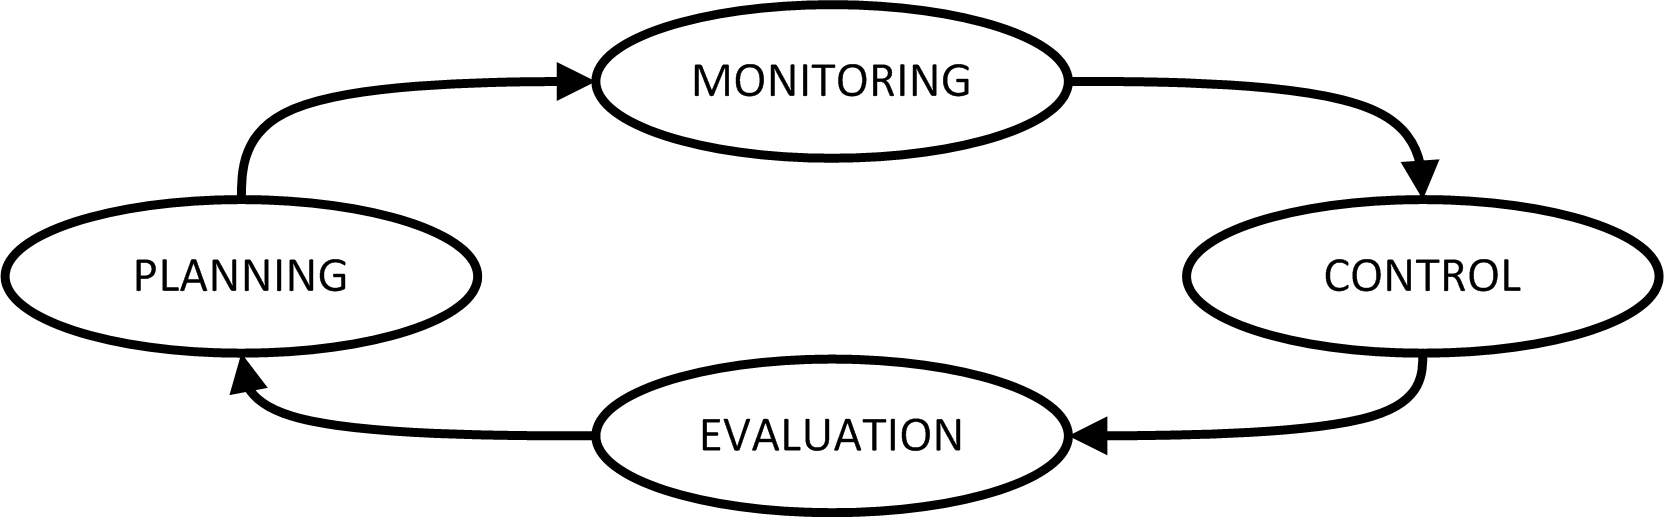
\includegraphics[width=1.0\columnwidth]{mission_management.png}
    \caption[Complete cycle in classic mission management]{Complete cycle in classic mission management.}
    \label{fig:mission_management}
\end{figure}

Thus flexible mission management includes the depicted four stages: mission planning, monitoring and control follows this. This is a
continuous cycle which runs indefinitely while the mission is active. This is a classic view of a Command and Control (C2) needs:

\begin{itemize}
  \item Planning: See the future - Audit trail of key mission planning and scheduling decisions providing a
  shared understanding of plan rationale and critical information justifying them.
  \item Monitoring: Feeling the present - Shared representation of assets and force package
  capabilities, including measures of performance (MoP) and effectiveness (MoE), but also task
  and mission progress and completion, especially for joint and cooperative operations.
  \item Control: Analyze the past - Validation of overall mission objectives (accomplished and
  non-accomplished), managing trade-offs of mission constraints and resource conflicts. These also
  include the communication of relevant commands and directives to mission forces at the right time.
\end{itemize}

Missions are high level specifications of (possibly) complex sequences of tasks to be achieved by the platforms of the system. The design of
a mission gives rise to a mission intent designed in a C2 station that can be potentially processed either centrally or in a distributed way,
so that each platform involved in the mission may be endowed with its own plan in terms of tasks and events. These platforms can evolve in
different environments such as air, terrain surfaces or water, and can be categorized in manned or unmanned or even according to their levels
of autonomy.

The platforms together with the payload on-board are the main elements to be considered in mission management scenarios. The interoperability
procedures for cooperative mission executed by a fleet of UAS are under the STANAG 4586. This standard establishes separated levels of
interoperability according to the type of mission, vehicles performances and payload capabilities. The payload has a very close relationship
with air vehicle, conditioning its nominal operation and strongly influencing the mission execution. Mission management is designed to
control and monitor both the air vehicle operations and also the payload performances, considering the payload as part of the vehicle.

\section{Global Architecture}
    \label{sec:global_architecture}

Depending on how accurate is the information about the mission to be performed, the future trajectory to be executed by the unmanned systems
can be described with different levels of detail. The trajectory is the result of performing the mission according to the goals and
objectives defined during the planning phase. These set of mission objectives is conditioned by the payload on-board, the type of mission to
be executed, the performances of the UAS and the environmental (mainly weather) conditions. The most precise information about all those
parameters implies more optimal planning and execution. In all cases, the mission information will be translated into an understandable set
of instructions that can be unambiguously interpreted by the UAS achieving the expected mission. Although this set of usable information
shall be structured according to the native input formats of each individual system, it is possible to define common structures that can be
used for synchronizing and data exchanging purposes. Based on the concept of interoperability, Boeing Research and Technology Europe has
defined two formal languages that are capable of encoding the trajectory information, the Flight Intent Description Language (FIDL) and the
Aircraft Intent Description Language (AIDL). Both are description of planned trajectories differentiated by the level of granularity
available for the trajectory identification. The former describes the foreseen trajectory by means of high level objectives and restrictions,
while the latter defines strictly the guidance modes to be executed by the Flight Control System (FCS) which ensure the aircraft is
adequately commanded. In the first case, the trajectory is not univocally described and a post processing is required for closing the degrees
of freedom that eventually could remain open. If the information does not leave any open degree of freedom, the trajectory is univocally
defined, and therefore, it can be formulated in terms of AIDL.

In this paper, these ideas are extended up to the mission level according to the global architecture depicted in Fig.~\ref{fig:global_arch}.
Three main components have been considered in descending level of abstraction: Mission Engine Infrastructure (MEI), Intent Generation
Infrastructure (IGI) and Trajectory Computation Infrastructure (TCI). Each component processes respectively the mission intent, the FIDL and
the AIDL.

In addition, another formal language called Payload Intent Description Language (PIDL) has been included in the architecture due to the
crucial role of the payloads on-board the UAS in the achievement of the goals in many missions and in the task allocation decision process,
i.e. which UAS should execute each task of the mission. The PIDL is processed by the Payloads Commands Generation Infrastructure (PCGI) that
generates the commands for the on-board payload in synchronization with the different segments of the trajectory computed by the TCI. As it
is shown in Fig.~\ref{fig:global_arch}, IGI, TCI and PCGI are close to the UAS at the conceptual level, although their software
implementations could be also executed in a centralized manner for a fleet of UAS.

Finally, the Performance Measurement Infrastructure (PMI) allows to check the execution against the expected effects encoded in the mission
intent. If there is any significant divergence during the mission, the PMI reports the detected contingency to the MEI, that replans the
required actions to manage that situation.

\begin{figure}
    \centering
    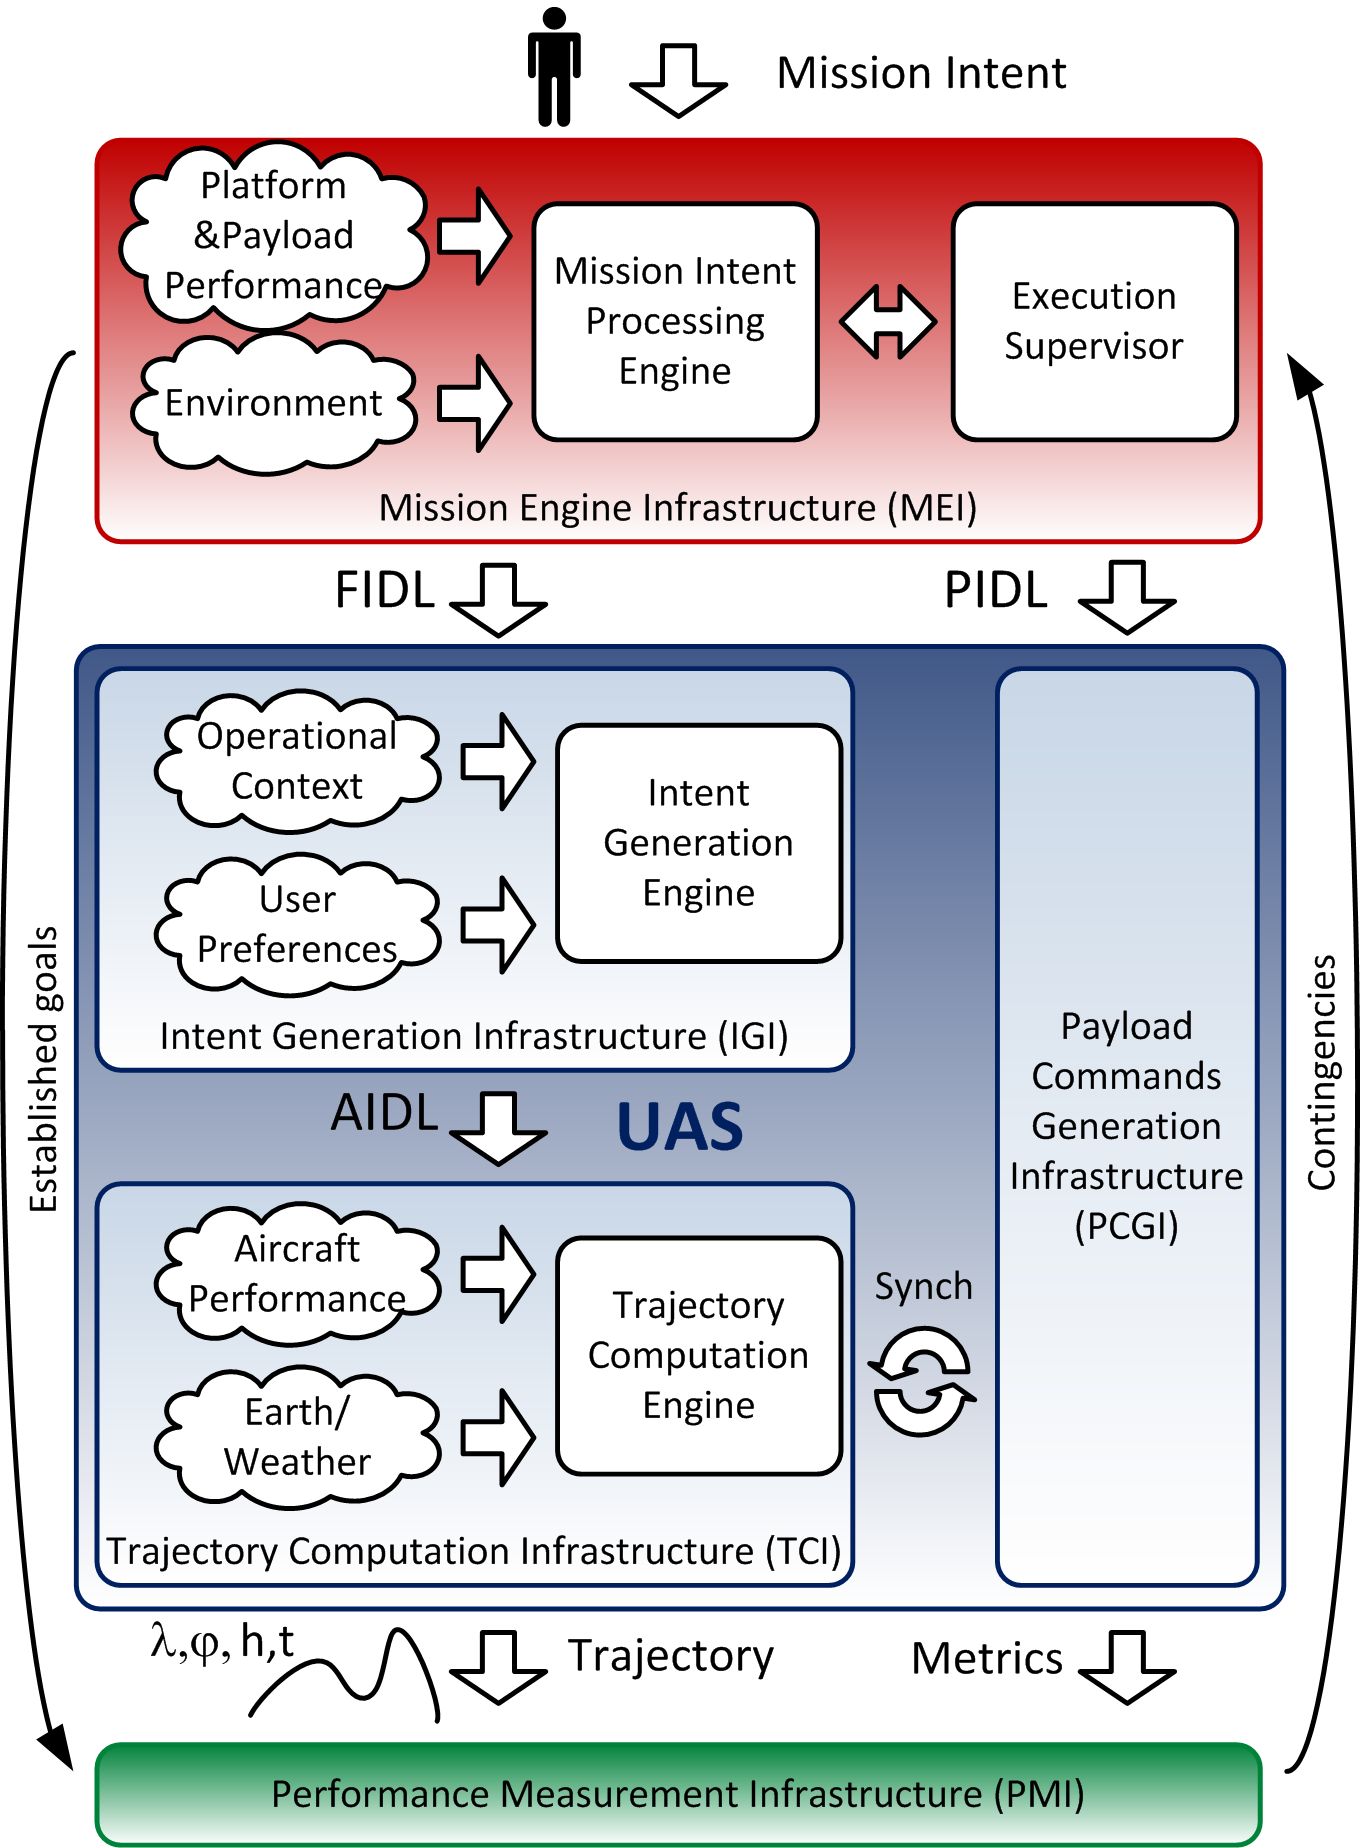
\includegraphics[width=1.0\columnwidth]{global_arch.png}
    \caption[Global architecture (only in planning phase)]{Global architecture (only in planning phase) extending the concepts of AIDL
    and FIDL up to the mission level. Three main components have been considered in descending level of abstraction: Mission Engine
    Infrastructure (MEI), Intent Generation Infrastructure (IGI) and Trajectory Computation Infrastructure (TCI). Each component
    processes respectively the mission intent, the FIDL and the AIDL. Another formal language called Payload Intent Description
    Language (PIDL) has been included in the architecture due to the crucial role of the payloads on-board the UAS in the achievement
    of the goals in many missions and in the task allocation decision process, i.e. which UAS should execute each task of the mission.}
    \label{fig:global_arch}
\end{figure}

The main components depicted in Fig.~\ref{fig:global_arch} are described in the following subsections.

\subsection{Mission Engine Infrastructure (MEI)}
    \label{sec:mei_description}

The output of this level is a set of messages encoded in different languages that will allow to define unambiguously the actions to be
executed by the platforms/payloads, and whose final outcome will be the achievement of the mission intent given as input. The MEI selects the
most appropriate platform according to the on-board payload and other factors, and generates the FIDL and PIDL instances that will describe
the operation of the platform and payload along the whole mission. The internal architecture and implementation details of the MEI are the
novel contribution of this paper and are summarized in Sect.~\ref{sec:MEI_architecture}.

\subsection{Intent Generation Infrastructure (IGI)}
    \label{sec:igi_description}

This level encompases all the algorithms and heuristics required for composing a message of AIDL using
as input a message of FIDL. As exposed above, the description of a trajectory can be represented in different ways
according to the detail available at the planning phase. This information, which should encode in a structured manner the
mission requirements, can be exhaustively precise or partially vague. If it is possible to describe the trajectory to be
executed without ambiguity, then it is possible to generate an AIDL message, otherwise the format selected should be the
FIDL because it allows leaving open some parameters to be closed afterwards. If this is the case, an additional process for
closing all undefined elements is required.

This process is performed by the Flight Intent Processing Engine which makes use of the additional information about user preferences and
operational context restrictions when available, or assumes predefined hypothesis to determine and fix the problem degrees of freedom. The
Operational Context Model is the IGI formal representation of any constraint and restriction related to the airspace where the flight will
take place (e.g., speed below 250kts within the terminal area or terrain obstacles). On the other hand, the Users Preference Model is the IGI
formal representation of the user preferences to be applied on the flight as operational procedures. This information can be translated into
certain trajectory constraints (e.g. cruise Mach) or into optimization criteria (e.g. minimum consumption).

\subsection{Trajectory Computation Infrastructure (TCI)}
    \label{sec:tci_description}

A trajectory computation infrastructure encodes the algorithms required for computing a trajectory based on the information related to the
aircraft intent and initial sate. It basically consists on the following three components:

\begin{itemize}
\item Aircraft Performance Model (APM) provides the means to predict aircraft performance characteristics, i.e. the aircraft response
under several (desirably any) motion and environmental conditions.
\item Earth/Weather Model allows predicting the atmosphere (temperature and pressure) and weather conditions (temperature and pressure
at sea level and wind) that the airplane would encounter as it executes the motion specified by the provided aircraft intent description,
as a function of spatial position, time and a set of parameters. These parameters may slightly evolve over time as environmental conditions change.
\item Trajectory Computation Engine computes the trajectory that the aircraft, performing as predicted by the corresponding APM,
would exhibit as a result of executing the specified aircraft intent description, starting from known initial conditions,
in presence of the environmental conditions given by the underlying environmental model. Computing the aircraft trajectory
does typically involve numerically solving a set of mathematical problems related to the integration of differential-algebraic
equations systems.
\end{itemize}


\section{Mission Engine Infrastructure Architecture}
    \label{sec:MEI_architecture}

Figure~\ref{fig:MEI_architecture} shows the system architecture of the Mission Engine Infrastructure (MEI) component and the details of its
relations with other components of the global architecture described in Sect.~\ref{sec:global_architecture}. Three main layers can be
identified from the top to the bottom of the figure: the mission intent syntax generator, the mission intent parser module and the MEI
component which generates FIDL sentences taking as input the mission intent specified by the operator.

\begin{figure}
    \centering
    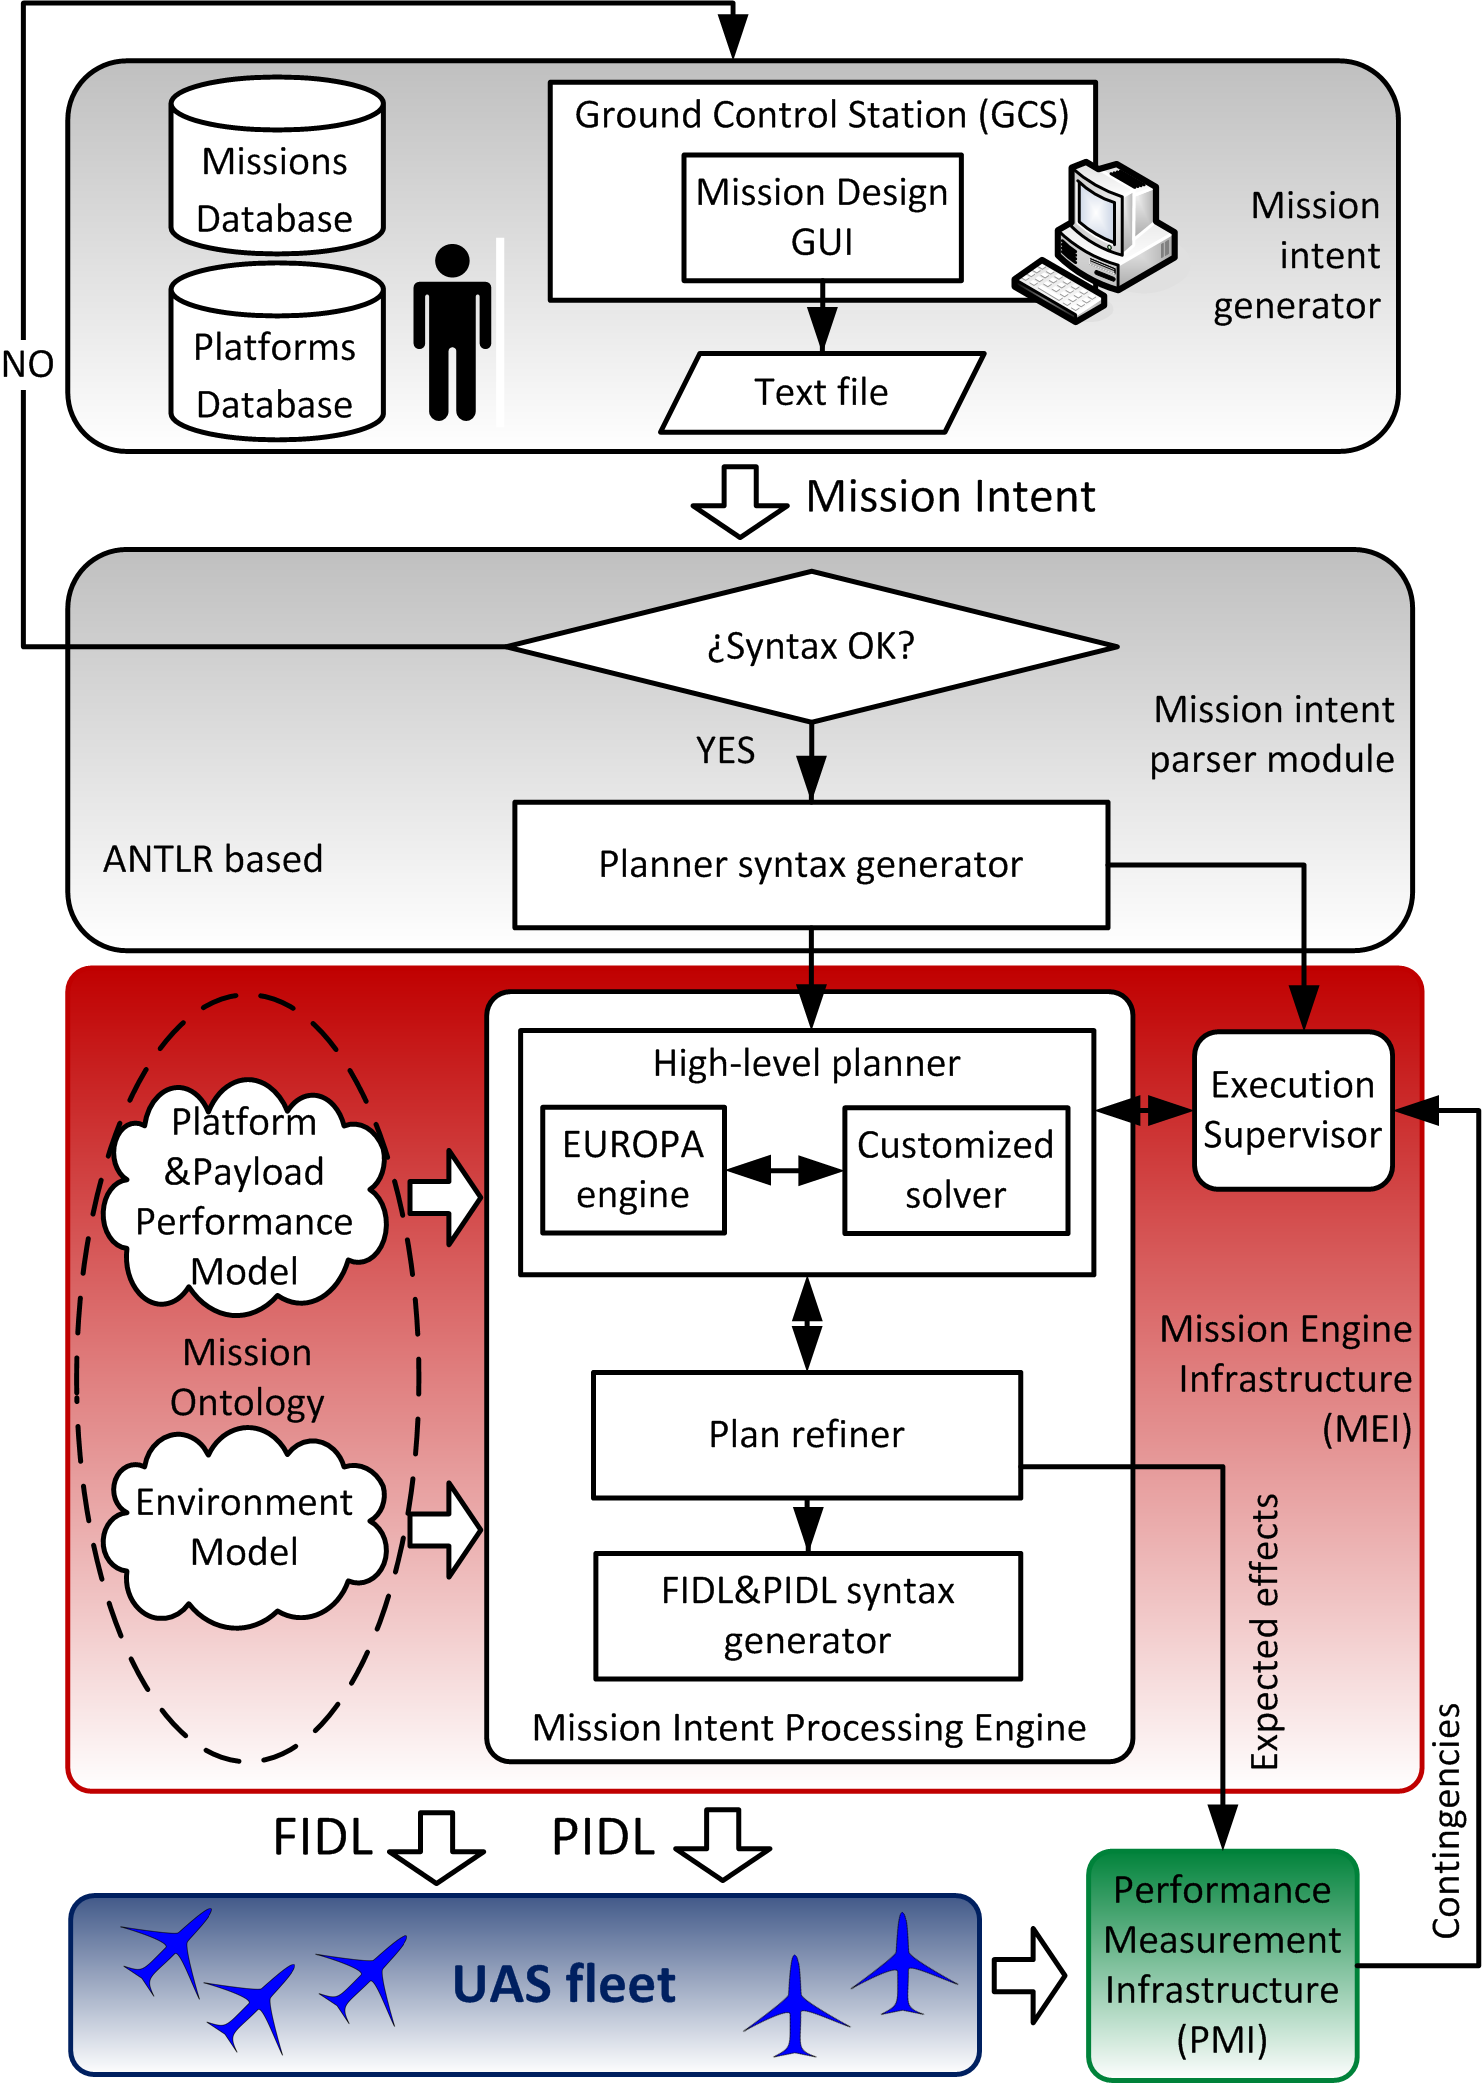
\includegraphics[width=1.0\columnwidth]{MEI_architecture.png}
    \caption[Mission Engine Infrastructure (MEI) architecture]{Mission Engine Infrastructure (MEI) component and the details of its
    relations with other components of the global architecture described in Sect.~\ref{sec:global_architecture}. Three main layers can
    be identified from the top to the bottom of the figure: the mission intent syntax generator, the mission intent parser module and
    the MEI component which generates FIDL sentences taking as input the mission intent specified by the operator.}
    \label{fig:MEI_architecture}
\end{figure}

The mission operator is depicted at the top level of the architecture in Fig.~\ref{fig:MEI_architecture} and has the responsibility of the
mission design by using any of the available mission intent syntax generators:

\begin{itemize}
\item A plain text editor to write all the sentences and save them in a mission intent file.
\item A friendly GUI (see Fig.~\ref{fig:midl_gui_syntax_generator}) that can assist the operator in the different steps of the mission
design process. For example the GUI allows the operator to define waypoints directly clicking on the map displayed in a Ground Control
Station (GCS) application~\cite{perez_jint13,maza_jint10_multimodal}. In this case, a mission intent file is automatically generated once the
design process is completed.
\end{itemize}

\begin{figure}
\centering
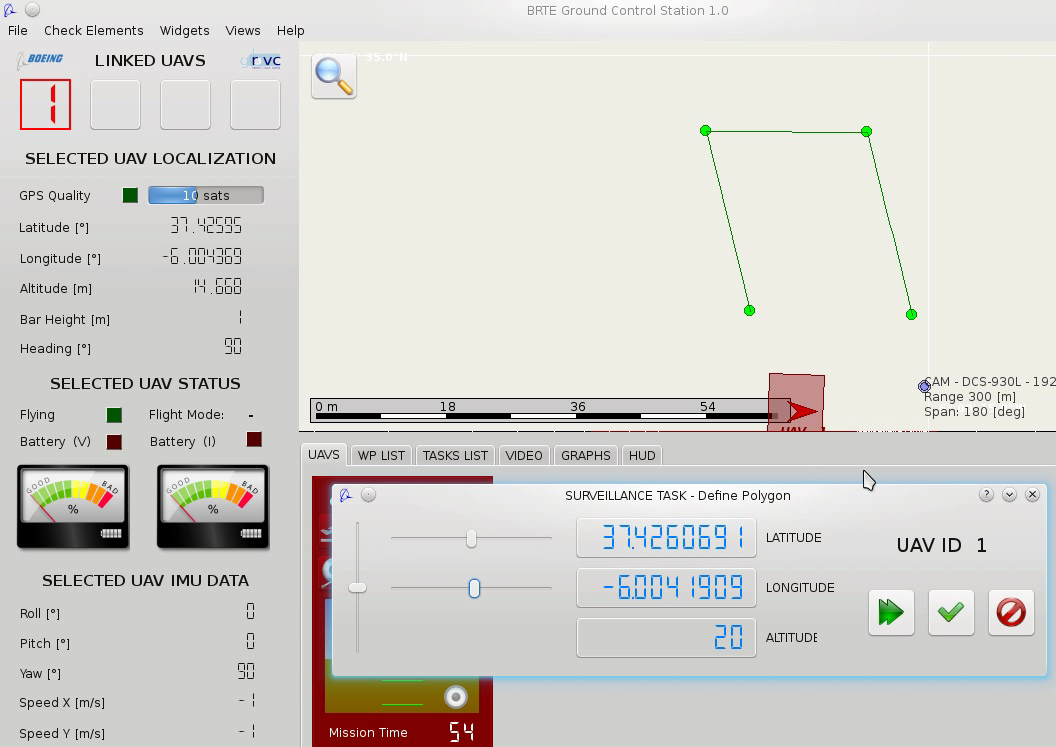
\includegraphics[width=1.0\columnwidth]{midl_gui_syntax_generator.png}
\caption[Graphical User Interface (GUI) of a Ground Control Station]{Graphical User Interface (GUI) of a Ground Control Station (GCS) with
an add-on intended to assist the operator in the mission design process.}
\label{fig:midl_gui_syntax_generator}
\end{figure}

In the next level, a parser based on ANTLR (ANother Tool for Language Recognition) \cite{antlr} checks the syntax of the mission intent
sentences generated in the previous level. If it is not correct, an error is reported and the user has to rewrite the wrong sentences. It
should be mentioned that a formal language has been developed in order to represent the mission intent. A bottom-up approach was followed:
the point of view of an user who wishes to design a mission involving possibly complex interactions between vehicles, making special emphasis
in the payload concept that will define the behaviour and utility of each vehicle and the interaction between them. The key idea of this
approach is to consider missions regarding the expected actions and results, instead of considering individually the point of view of each
involved vehicle that would lead to a rigid and un-adapted description of the missions. The following requirements were considered in the
design of the language used to describe the missions:

\begin{itemize}
\item Define completely and unambiguously the mission intent.
\item Describe univocally the high level mission objectives with or without defining the final performance of vehicles and payloads for
achieving the mission.
\item Include the required information that support the processes of automation and automatic initiative, network centric operations and
collaboration and cooperation between platforms in joint operations.
\item A formal language to be interpreted by the MEI component.
\end{itemize}

The definition of the formal language was done with the assistance of ANTLR, which is a language tool that provides a framework for
constructing recognizers, compilers, and translators from grammatical descriptions containing actions in a variety of target of languages
(Java, C, C++, ADA, Python, PHP, Perl, etc). ANTLR is widely used because it is easy to understand, powerful, flexible, generates
human-readable output, comes with complete source under the BSD license, is actively supported, and usually allows writing actions in
different languages. Within ANTLR, the ANTLRWorks tool (see Fig.~\ref{fig:antlrworks}) generates graphical feedback showing the rules during
the design/building process of the different sentences.

\begin{figure}
    \centering
    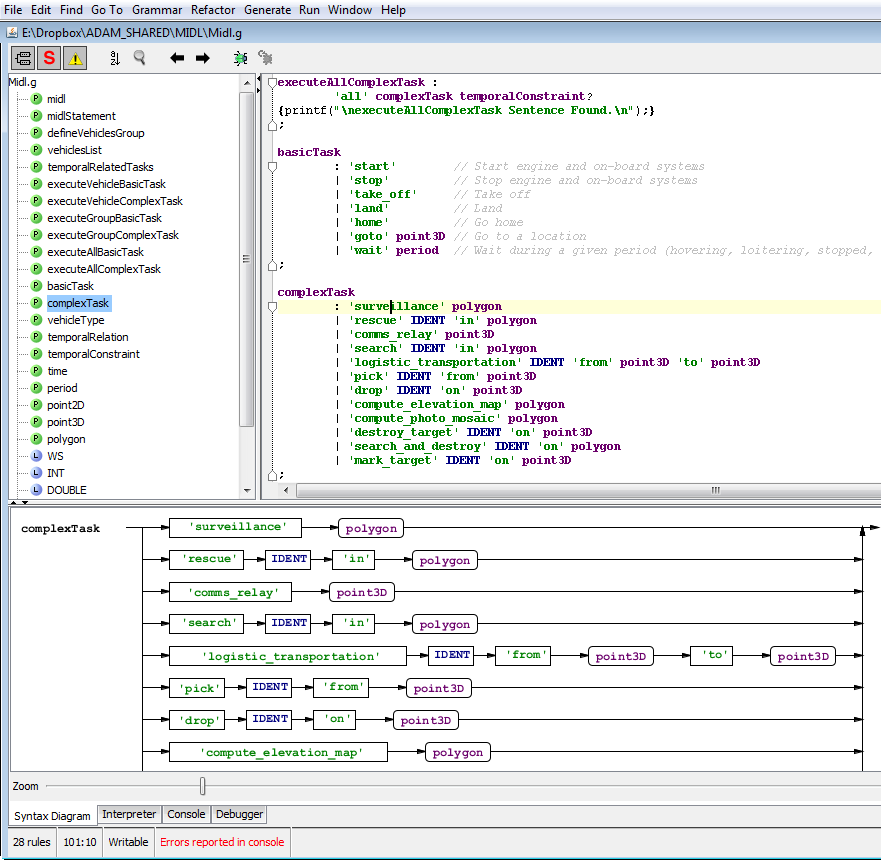
\includegraphics[width=1.0\columnwidth]{ANTLRWorks.png}
    \caption[ANTLRWorks screenshot. The syntax is shown on the subwindow above and the subwindow
    below shows graphically the rule corresponding to the sentence]{ANTLRWorks
    screenshot. The syntax is shown on the subwindow above and the subwindow below shows
    graphically the rule corresponding to the sentence.}
    \label{fig:antlrworks}
\end{figure}

Once the ANTLR parser has determined that the sentences of the mission description are correct, the planner syntax generator processes the
mission intent sentences and translates them into the format used by the planner endowed in the MEI in the next level. The output of this
component is a set of messages encoded in different languages that will allow to define unambiguously the actions to be executed by the
platform and the payload, and whose final outcome will be the achievement of the established mission. The MEI module will be in charge of
selecting the most appropriate platform with its on-board payload and to generate the FIDL and PIDL instances that will describe the
operation of the platform and payload along the whole mission.

The MEI is composed by the models and knowledge database (mission ontology), an execution supervisor and the Mission Intent Processing Engine
(MIPE). These elements are described in the next subsections.

\subsection{Mission Intent Processing Engine (MIPE)}
    \label{sec:mipe}

The EUROPA (Extensible Universal Remote Operations Planning Architecture) planner \cite{europa} is currently used as the core component of
the Mission Intent Processing Engine (MIPE) as it can be seen in Fig.~\ref{fig:MEI_architecture}. It that takes as input the parsed mission
intent sentences and generates a high-level plan in a multi-vehicle context. This planner computes feasible plans satisfying the different
temporal constraints specified in the mission.

The EUROPA framework was developed at NASA's Ames Research Center and is a class library and tool set for building planners (and/or
schedulers) within a Constraint-based Temporal Planning paradigm. Constraint-based Temporal Planning (and Scheduling) is a paradigm of
planning based on an explicit notion of time and a deep commitment to a constraint-based formulation of planning problems. EUROPA is now in
the second version and is the successor of the original EUROPA which in turn was based upon Heuristic Scheduling Testbed System (HSTS)
\cite{muscettola98remote}.

EUROPA is designed to be expressive, efficient, extendable and configurable, and includes the following components:

\begin{itemize}
\item\textbf{A plan database:} The technology cornerstone of EUROPA for storage and manipulation of plans as they are initialized and
refined. This database integrates a rich representation for actions, states, objects, resources and constraints with algorithms for automated
reasoning, propagation, querying and manipulation. This representation allows concise declarative descriptions of problem domains and
powerful expressions of plan structure. It is supported with a language for describing problem domains and data structures for instantiating
and manipulating problem instances. This language called NDDL (New Domain Definition Language) \cite{Frank02,Bernardini07} is a very
high-level, object-oriented, declarative domain and problem description language. For instance, this language allowed us to describe the
mission ontology presented in Sect.~\ref{sec:ontology} composed by the platforms, payloads and environment models (see
Fig.~\ref{fig:MEI_architecture}). The NDDL representation includes state and activity descriptions, as is common in planners using
traditional modelling languages like the Planning Domain Definition Language (PDDL) \cite{Gerevini09,Hoffmann05}. However, unlike PDDL, NDDL
uses a state variable value formalism. EUROPA thus takes its heritage from planning formalisms like IxTeT \cite{Ghallab94} and SAS+
\cite{Jonsson98}.

\item\textbf{A problem solver:} A core solver to automatically find and fix flaws in the plan database. It can be configured to plan,
schedule or both, and includes a component-based architecture for flaw identification, resolution and heuristics as well as an algorithm for
chronological backtracking search. It can be easily customized to integrate specialized heuristics and resolution operations.

The EUROPA solver stops once it finds a feasible plan, but it does not perform any optimization based on mission performance metrics. Hence
a customized solver module should be developed for the type of missions considered. In addition, some costs should be associated to the
different tasks to be executed during the mission and the association has to be done externally to the EUROPA framework.

\item\textbf{A tool box:} EUROPA includes a debugger for instrumentation and visualization of applications. It also includes a very
high-level, declarative modelling language for describing problem domains and partial-plans. In particular, EUROPA incorporates several tools
that allows the user to drive EUROPA interactively by making use of its PSEngine client interface, and a number of prepackaged UI components
(PSGantt, PSChart, PSSolverDialog, ActionDetails and ActionViolation). These tools have been used to show some planning results in
Sect.~\ref{sec:example}.
\end{itemize}

The EUROPA framework allows developing specific planners and/or schedulers under constraint reasoning in order to integrate them into an
end-user application. It is designed to be open and extendable to accommodate diverse and highly specialized problem solving techniques
within a common design framework and around a common technology core. Then EUROPA represents a reasonable choice as the core engine of the
MIPE.

The resulting computed plan is composed by high-level tasks that might require some refinement to make them consistent with the
parameters that should be present in the FIDL sentences. The plan refiner module is required to adapt the high-level plan computed by EUROPA
into a plan closer to the level of abstraction managed by the FIDL level. It computes the values required in FIDL that might have not been
previously grounded in the planning process.

Finally, the FIDL\&PIDL syntax generator software module generates a XML file with the flight/payload intents in a format that can be
processed by the next level (IGI and PCGI) in the global architecture depicted in Fig.~\ref{fig:global_arch}.

\subsection{Mission Ontology}
    \label{sec:ontology}

An ontology formally represents a set of concepts within a specific domain (in this case mission specification), and the relationships
between those concepts. It can be used to reason about the entities within a domain and may be used to describe the domain. Ontologies
provide standards not only for data within a specific domain, but also for the processes that use such data. For instance, mission management
ontology should include data models that describe mission activities, and also explicit representations of the mission management processes
and how information is used and updated within those processes.

As it can be seen in Fig.~\ref{fig:MEI_architecture}, the basic components of the mission ontology are the platform, payload and environment
models:

\begin{itemize}
\item The platform performance model describes the platforms involved in a specific mission. Platform, in this
architecture, is understood as a vehicle (with or without autonomous abilities) able to contain a payload on-board. This ontology has all the
vehicles as instances. Every instance will have specific attributes, for example: mode (air, terrain, and sea), maximum velocity, payload
restrictions (volume and weight), autonomy, communication capabilities on-board and available protocols to communicate, etc.

\item The payload performance model describes the possible payloads involved in a specific mission. This payload could be
installed in a set of possible platforms in order to develop some specific actions in a mission, such as identifying, detecting, tracking,
etc. Each payload could be performing different tasks according to its capabilities and the limitations of the complete system
platform-payload. The payloads listed in the STANAG 4586 have been considered at this point of the development: EO, IR, EO/IR, SAR, fixed camera, communication relay, dispensable payload, recorder and payload bay door. However, in order to increase the spectrum of possible missions it is also interesting to include other payloads, such as object transportation and deployment devices \cite{maza_jfr11_transportation}.

\item The environment model endows the ground and airspace models.

The former contains data about the ground surface related to the mission: object detection, mapping, alarm monitoring, etc. The ground can be
represented by a 2-dimensions array of cells. Each cell represents a piece of the ground, and have a square shape projection onto a
horizontal plan. In order to describe this world, several attributes can be associated to each cell: the current quality of mapping, the
latest date of mapping, the latest date of object detection, etc.

On the other hand, the airspace model contains data about airspace, which give relevant information to plan trajectories at the level of
waypoints (as it was mentioned before, the granularity of the trajectories increases through the levels of the FIDL and AIDL). In a first
stage, a discrete airspace model is considered. The atmosphere is represented by a 3D array of regular voxels, that are not necessarily
cubic, nevertheless it seems obvious that the basis of the voxels is square. In order to describe this world, several attributes can be
associated to each voxel: state of traversability, a vector with the wind inside, etc. From this first stage, an airspace graph can be
generated with nodes which are potential waypoints, and edges labeled with the cost for the UAS to move from one node to an adjacent node. Finally, it can be useful to have an area model. An area is only a way to reference a given area as a whole, instead of enumerating every cell that composes it.

\end{itemize}

The different models introduced here are intended to enable the manipulation of the knowledge in the decision framework presented in
Sect.~\ref{sec:mipe}. These models can be exploited by the different vehicles, within their own plan refiners and supervisor components,
whenever the higher levels of decisional autonomy are requested.

\subsection{Execution Supervisor}
    \label{sec:supervisor}

As it was mentioned before, missions are high level specifications of (possibly) complex sequences of tasks to be achieved by the vehicles of
the system. The design of a mission gives rise to a mission specification that can be potentially processed either centrally or in a
distributed way, so that each vehicle involved in the mission may be endowed with its own plan in terms of tasks and events.

However, during the execution of any mission it is very likely that contingencies may occur. Planning must be flexible and must include the
uncertainty environment of actions. For example, air operations should be executed according to an Air Tasking Order (ATO), which may take up
to 72 hours to plan, task and execute. In volatile situations, information about the vehicle's operating environment may be limited.
Therefore, task planning flexibility and safe trajectory solutions are essential to the survivability and success of an autonomous system.
The vehicle's guidance and mission planning systems must possess enough intelligence (and processing power) to recognize and react to changes
in the operating conditions. On the other hand, if the vehicle is ordered to perform a new mission task during an operation, it must possess
the capability to safely transition from its previous trajectory to its new mission goals.

Task processing is identified at the logical level through partially ordered events sequence: every task first triggers a  start � event when
launched, then an  end � event when (correctly) ending. Only the  start � event can be controlled: the  end � event is contingent, from the
point of view of the users of the system, as well as any other event that may occur during the task execution.

A task is characterized by a temporal extent: the lapse of time between the  start � event and the  end � event. Depending on the
task, this lapse of time can be approximately assessed, but as far as the  end � event is contingent, the exact temporal extent of a task
can usually be known only when the task is completed.

The low level part of the supervisor is intended to supervise the tasks while they are being executed (tracking their status of evolution)
and to manage simple contingent events that may occur according to according to the so-called built-in rules, as it is shown on
Fig.~\ref{fig:basic_tasks_and_events}. Several tasks can be triggered or executed in parallel. However only one running instance of a
particular task is allowed in a vehicle. This restriction should be corrected whenever the need for running several instances of the same
task within one vehicle arises. The tasks requested may be pending if some of their preconditions are not satisfied yet: this mechanism fits
the needs for sequences of tasks, when each task of a sequence is waiting for the previous one to end its execution. This end of execution
triggers an event that matches the un-satisfied precondition of the following task, hence this following task is itself triggered, and so on.

\begin{figure}
\centering
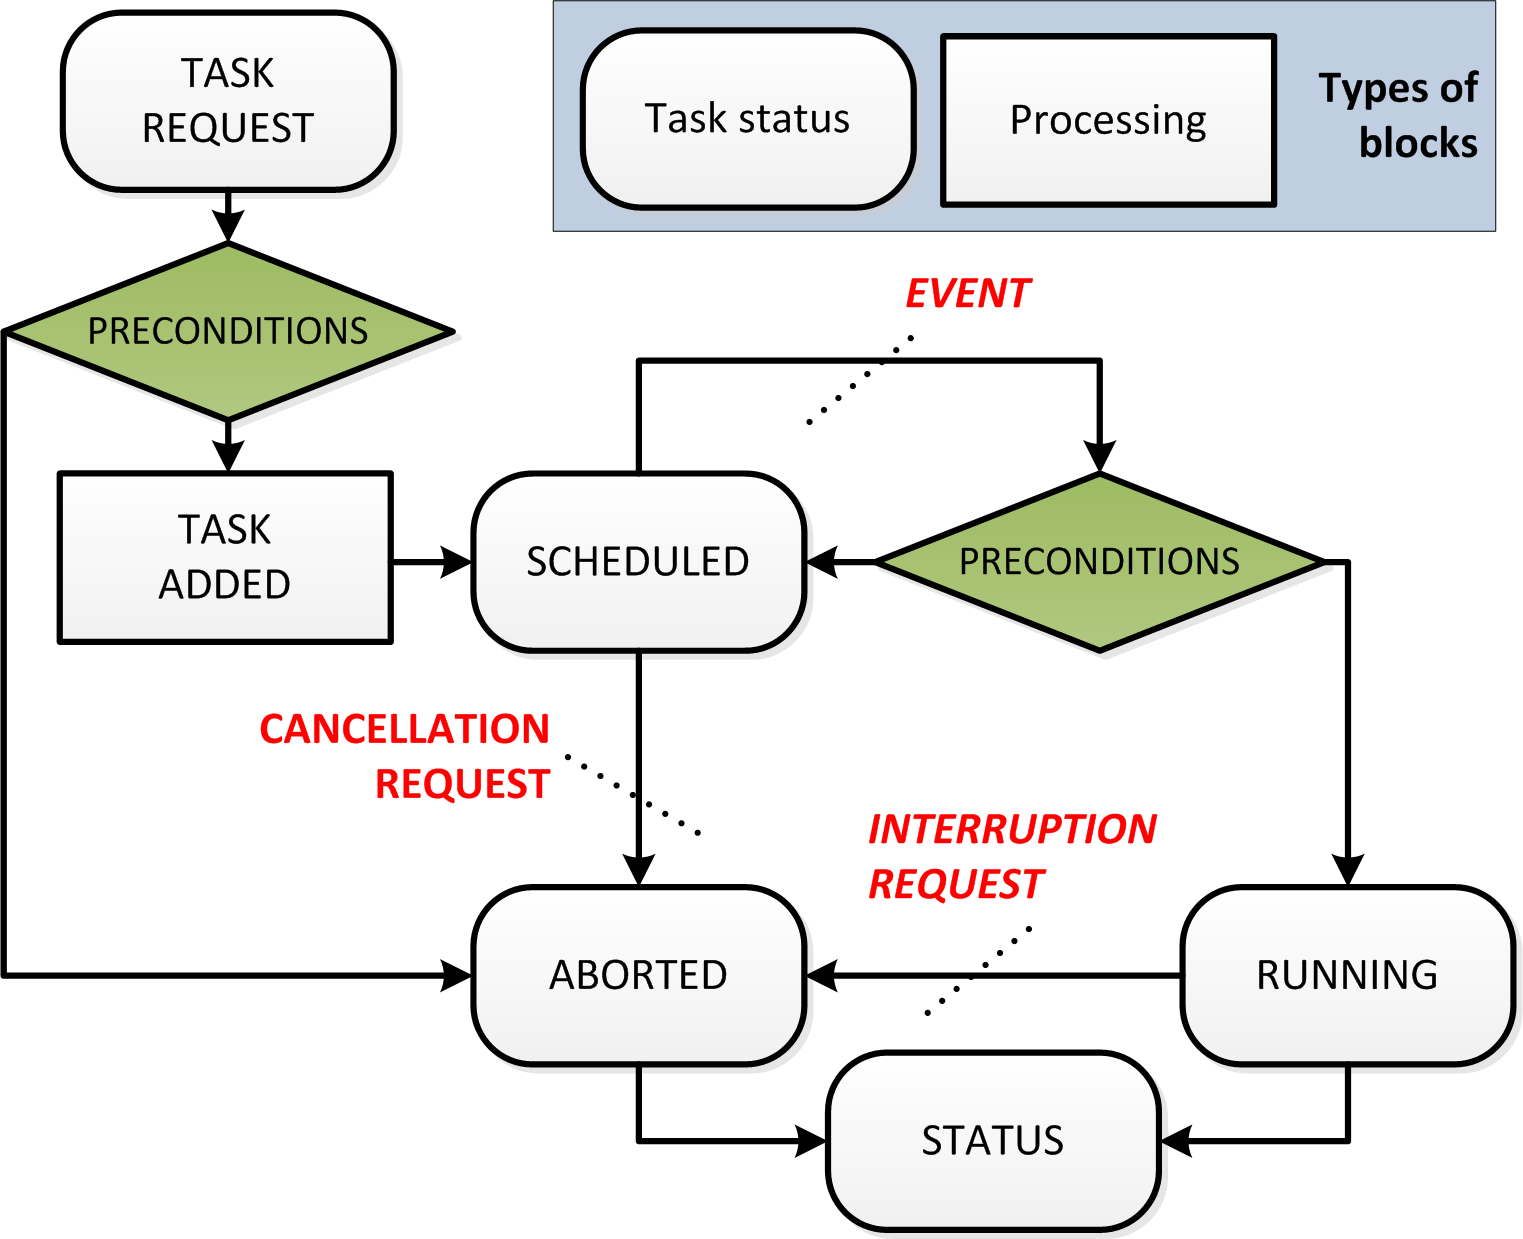
\includegraphics[width=0.9\columnwidth]{basic_tasks_and_events.png}
\caption[Built-in rules and events management within the supervisor]{Built-in rules and events management within the supervisor.}
    \label{fig:basic_tasks_and_events}
\end{figure}

As an additional feature, in the mission intent definition it has been considered useful to allow the operator to specify rules with the
desired behaviour for the platforms in response to different possible contingencies. These rules are passed directly to the supervisor from
the planner syntax generator (see Fig.~\ref{fig:MEI_architecture}) and are added to the built-in rules. The supervisor also interacts with
the high-level planner for re-planning purposes if it is required.

\section{An Example: Surveillance Mission}
    \label{sec:example}

In this section, a representative mission such as surveillance will be used to illustrate the operation of the Mission Engine Infrastructure
in a multi-vehicle context. In this mission, several UAVs are available with the following types of payloads: EO, IR and EO/IR cameras. The complete fleet of vehicles is composed by 5 UAVs (quadrotors) and 3 UGVs. On the other hand, different time slots in a single day are
considered depending on the available natural light in the geographic area where the mission has to be executed: dawn (6:00--8:00), day (8:00--19:00), late afternoon (19:00--21:00) and night (21:00--6:00).

Listing~\ref{intent_example} shows the mission intent specified by the user: basically to start a surveillance task at 20:35 on a given area called \verb+delta_area+ in order to find intruders with likelihood 75\% and then return home. The user also included a contingency that generates a rule directly for the execution supervisor.

\lstinputlisting[label=intent_example,caption=Mission intent: start a surveillance task at 20:35 on a given area.]{midl_mission_example.txt}

In order to illustrate how to approach modelling application domains in the EUROPA framework, a batch application has been created providing
an application domain model and problem definition to the planner. The planner must then generate a plan to solve the problem.
Figure~\ref{fig:europa_batch_planning} shows the main inputs and outputs of our application.

\begin{figure}
\centering
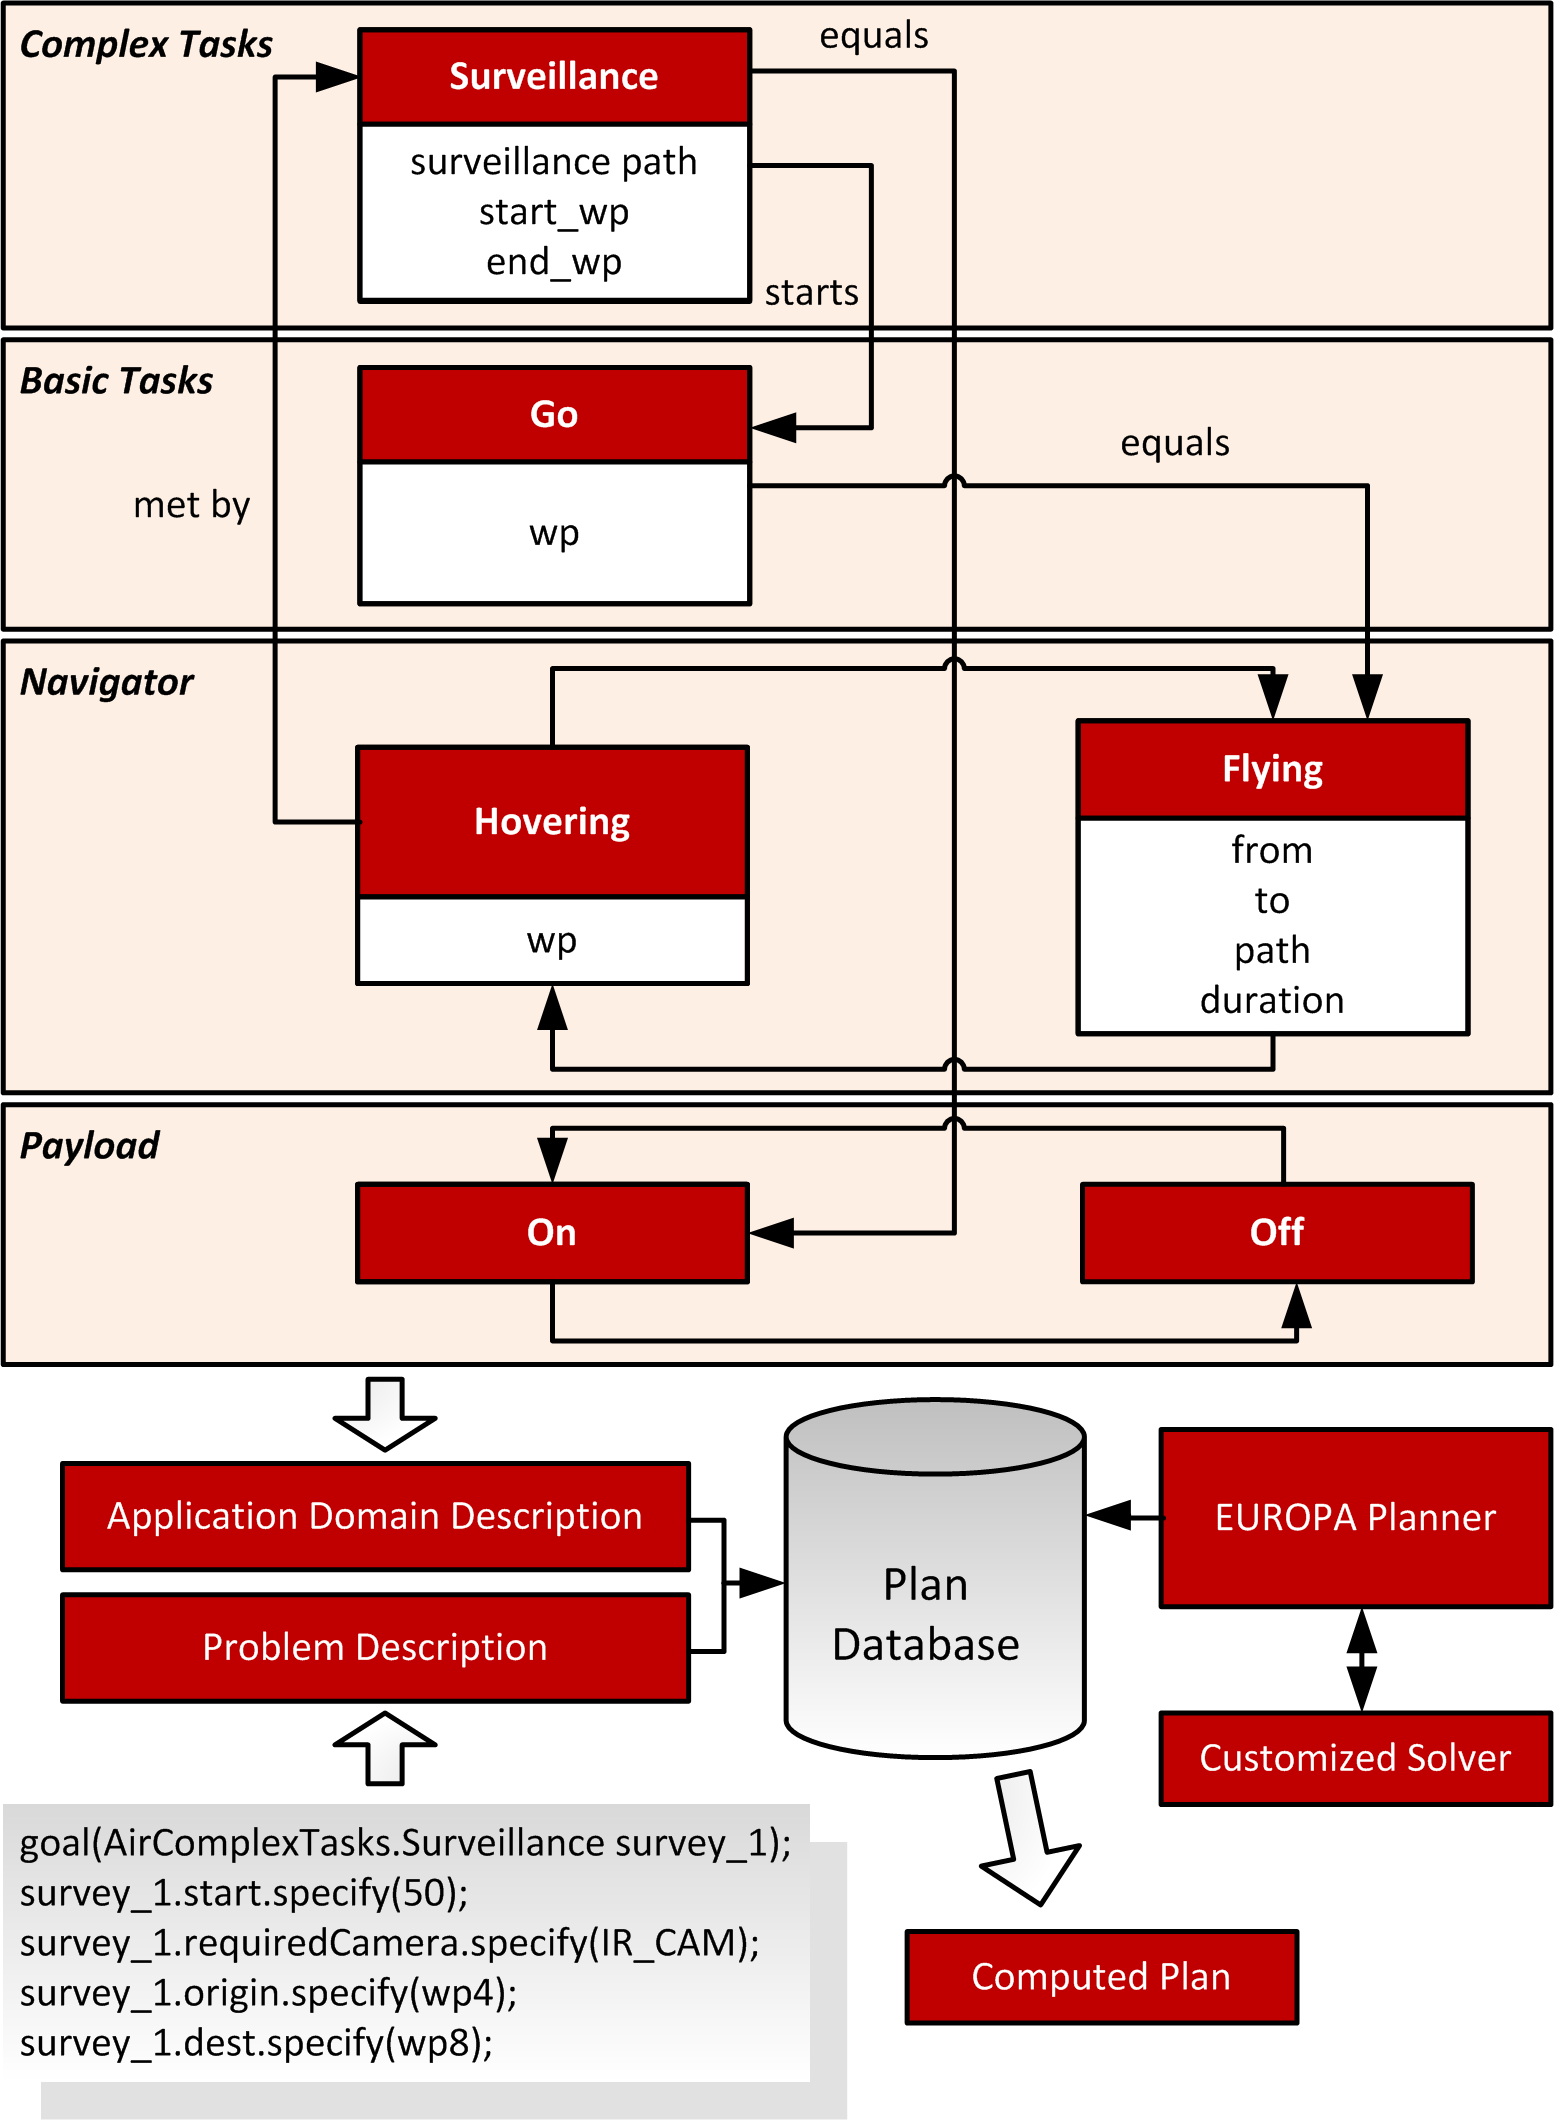
\includegraphics[width=1.0\columnwidth]{europa_batch_planning.png}
\caption[Scheme of the batch planning application under EUROPA used to plan the surveillance mission]{Scheme of the batch planning application under EUROPA used to plan the surveillance mission.}
    \label{fig:europa_batch_planning}
\end{figure}

In this example, the main entity in our application domain is the quadrotor. The next decision is to identify the entities, called timelines
in the following, that will describe changes in state of the quadrotor as it moves around the environment performing a mission. The quadrotor
in our domain is the actor for which the planning is done and which contains all the timelines. The next stage is to identify the states
(called predicates) that each timeline can be in. The easiest way to identify the predicates is to think through the lifecycle of each
timeline.

The set of predicates identified on each timeline along with the variables in each state for the quadrotor are shown on top of
Fig.~\ref{fig:europa_batch_planning}:

\begin{itemize}
\item Navigator: controls the motion of the quadrotor between locations and hovers at a location. Then, the vehicle can be
hovering at a location or going between locations.
\item Payload: controls the on-board payload that can be on or off.
\item Basic tasks: manages basic tasks. For example, the quadrotor can be instructed to go to a given waypoint.
\item Complex tasks: manages complex tasks. For instance, the quadrotor can be commanded to perform surveillance on a given area.
\item The meanings of the state transitions added to this figure are intuitive. It can transition
only to a new state connected in our diagram by an arrow. The next stage is to consider the constraints between predicates on different
timelines. So far we have only used the notion of state transitions to connect predicates; these map to the temporal relations of
\verb+meets+ and \verb+met by+ and are sufficient for timelines where only one predicate instance can occur at any given moment. When
predicates are connected between timelines, it is required to use the full range of temporal relations as concurrent states appear. In our
diagram, only \verb+met by+, \verb+starts+ and \verb+equals+ temporal relations according to \cite{allen_1983} have been considered.
\end{itemize}

Then, the application domain description is encoded in NDDL (New Domain Description Language). The description contains the so-called AirVehicle class which pulls together all the components previously defined. It has an attribute for the navigator, payload, basic tasks, complex tasks and battery classes. The constructor takes an instance of the built-in Battery class and creates instances of the other classes to setup the quadrotor. On the other hand, the initial state of the domain is also encoded in NDDL. It contains the specific locations of the waypoints involved in the mission, the initial location and battery level of the quadrotors and the different paths (with their associated costs computed by the plan refiner component) between the locations of interest.

Finally, the goal of the mission is computed automatically from the mission intent specified in Listing~\ref{intent_example} and the
resulting file encoded in NDDL is shown at the bottom of Fig.~\ref{fig:europa_batch_planning}. With the model and the initial state
specified, the planner can be started to compute the solution. Figure~\ref{fig:gantt} shows the Gantt chart computed by EUROPA for the
different timelines that represent .

\begin{figure}
\centering
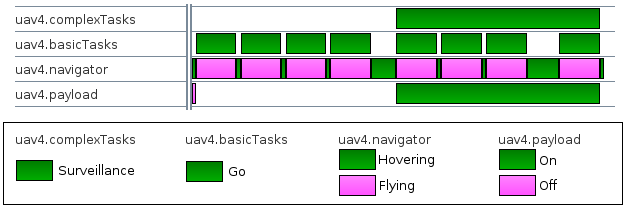
\includegraphics[width=1.0\columnwidth]{gantt.png}
\caption[Gantt chart computed by EUROPA for the different timelines]{Gantt chart computed by EUROPA for the different timelines.}
    \label{fig:gantt}
\end{figure}

The MEI module analyzes the different possibilities taking into account the scheduling of the mission and the capabilities of the vehicles
according to their payloads. It generates a sequence of basic tasks (type goto) that are translated into
the FIDL syntax in a file composed by several flight segments (see Listing~\ref{fidl_example}).

\lstinputlisting[label=fidl_example,caption=Resulting file in XML with the FIDL sentences required to achieve the surveillance mission.]{fidl_example.xml}

\section{Conclusions and Future Work}
\label{sec:conclusions}

This paper has described the software architecture and tools used to generate the Flight Intent Description Language (FIDL) sentences that
will command different aerial vehicles in order to execute a given mission specified by the operator. This architecture allows dealing with
the heterogeneity of the vehicles and missions to be executed.

A mission intent syntax generator, a mission intent parser module and the MEI component which generates FIDL sentences taking as input the
mission intent specified by the operator have been also described. The criteria used to design a mission intent language and the ANTLR tools
used to define it and to generate a parser for this language have been provided. However, this mission intent language is still under development according to the specifications mentioned in Sect.~\ref{sec:MEI_architecture}.

Regarding the MEI architecture, different components have been identified: the models and knowledge database (mission ontology), an execution
supervisor and the Mission Intent Processing Engine (MIPE). The latter component relies mainly on the EUROPA planner that takes as input the
parsed mission intent sentences and generates a high-level plan in a multi-vehicle context. Feasible plans satisfying
the different temporal constraints specified in the mission are computed, but once a plan is found, the engine stops. Then, future work should include the development of customized solvers for EUROPA intented to optimize the solutions computed.

%-----------------------------------------------------------------------------
% ACKNOWLEDGMENTS
%-----------------------------------------------------------------------------
\section{Acknowledgments}

The authors would like to thank the \emph{Boeing Research \& Technology Europe} company for their financial and technical support.

%-----------------------------------------------------------------------------
% BIBLIOGRAPHY
%-----------------------------------------------------------------------------
\bibliographystyle{IEEEtran}
\bibliography{IEEEabrv,bibliography}

\end{document}

%\begin{table}
%\caption{An Example of a Table}
%\label{table_example}
%\begin{center}
%\begin{tabular}{|c||c|}
%\hline
%One & Two\\
%\hline
%Three & Four\\
%\hline
%\end{tabular}
%\end{center}
%\end{table}
